\documentclass[12pt,a4paper]{article}
\usepackage{amsmath, amssymb, geometry, booktabs, xcolor, hyperref,
            listings, pgfplots, tcolorbox, enumitem, fancyhdr, tikz, array}
\geometry{margin=2.5cm}
\pgfplotsset{compat=1.18}
\tcbuselibrary{skins, breakable}
\usetikzlibrary{positioning, shapes.geometric}

% ── tcolorbox environments ──────────────────────────────────────────────────
\newtcolorbox{curiositybox}[1]{colback=yellow!10, colframe=orange!80!black,
  fonttitle=\bfseries, title={#1}, breakable}
\newtcolorbox{infobox}[1]{colback=blue!5, colframe=blue!60!black,
  fonttitle=\bfseries, title={#1}, breakable}
\newtcolorbox{mistakebox}[1]{colback=red!5, colframe=red!60!black,
  fonttitle=\bfseries, title={#1}, breakable}
\newtcolorbox{learnbox}[1]{colback=green!5, colframe=green!60!black,
  fonttitle=\bfseries, title={#1}, breakable}

% ── lstlisting (Python) ─────────────────────────────────────────────────────
\lstset{language=Python, basicstyle=\ttfamily\small, keywordstyle=\color{blue},
        commentstyle=\color{gray}, stringstyle=\color{orange},
        showstringspaces=false, numbers=left, numberstyle=\tiny,
        breaklines=true, frame=single}

% ── fancyhdr ────────────────────────────────────────────────────────────────
\pagestyle{fancy}
\fancyhf{}
\lhead{Topic 05: Applications to ODEs}
\rhead{Unit V --- Inverse Laplace Transforms}
\cfoot{\thepage}

% ── Title ────────────────────────────────────────────────────────────────────
\title{Topic 05: Applications to Ordinary Differential Equations \\
       \large Unit V --- Inverse Laplace Transforms}
\author{ \\
        JNTUA College of Engineering (Autonomous) ATP}
\date{}

% ─────────────────────────────────────────────────────────────────────────────
\begin{document}
\maketitle
\tableofcontents
\newpage

% =============================================================================
\section{Opening Hook}
% =============================================================================
\begin{curiositybox}{Hook}
Two full units. Twelve topics in Unit IV, five topics in Unit V. You have learned
the definition, existence conditions, all standard transforms, five operational
properties, derivatives, integrals, multiplication and division by $t$, evaluation
of integrals, inverse transforms, partial fractions, and convolution. All of it has
been building toward one destination: solving ordinary differential equations that
arise in electrical circuits, mechanical systems, control engineering, and heat flow.
This is that destination. In this topic, you will solve ODEs that would take pages
using classical methods --- each solved in under half a page using the Laplace
Transform. Let's go.
\end{curiositybox}

% =============================================================================
\section{Why This Topic Exists}
% =============================================================================

Before we begin, here is the honest answer to why you are reading this. The Laplace
Transform method does something no classical technique can match: it converts an ODE
together with its initial conditions into a pure algebraic equation in $s$. You solve
for $Y(s)$, apply one of the four inversion methods you have now mastered, and the
solution $y(t)$ appears directly --- with initial conditions automatically absorbed.

More importantly, the method handles \emph{discontinuous} and \emph{impulsive} forcing
functions --- unit steps and Dirac deltas --- with the same ease as smooth forcing.
The table below shows what happens when students skip the foundations.

\medskip
\begin{center}
\begin{tabular}{@{}p{7cm}p{7cm}@{}}
\toprule
\textbf{Mistake} & \textbf{Consequence} \\
\midrule
Skipping Units IV--V and going directly to the ODE solutions &
No understanding of \emph{why} each step works --- just following a recipe \\
\midrule
Forgetting to substitute initial conditions before inverting &
Getting the wrong particular solution without ICs \\
\midrule
Not recognising which inversion method to use &
Stuck at $Y(s)$ --- cannot recover $y(t)$ \\
\bottomrule
\end{tabular}
\end{center}
\medskip

\begin{learnbox}{Key Insight}
The Laplace Transform converts the IVP problem into algebra. Initial conditions are
not patched on afterward --- they are built into the algebraic equation from Step 1.
This is the single greatest advantage of the method.
\end{learnbox}

% =============================================================================
\section{The Universal 4-Step Workflow}
% =============================================================================

\begin{infobox}{The Complete Laplace ODE Algorithm}
Apply this four-step process to every ODE in this topic.

\bigskip
\textbf{Step 1: Apply $\mathcal{L}$ to both sides of the ODE.}

Use the derivative formulas:
\begin{align}
\mathcal{L}\{y'\}   &= sY(s) - y(0) \nonumber \\
\mathcal{L}\{y''\}  &= s^2Y(s) - sy(0) - y'(0) \nonumber \\
\mathcal{L}\{y'''\} &= s^3Y(s) - s^2y(0) - sy'(0) - y''(0) \nonumber
\end{align}

\textbf{Step 2: Substitute the given initial conditions} $y(0)$, $y'(0)$, etc.
The equation is now purely algebraic in $Y(s)$ and $s$.

\textbf{Step 3: Solve for $Y(s) = \mathcal{L}\{y(t)\}$} algebraically (collect $Y$
terms, factor, divide).

\textbf{Step 4: Invert $Y(s)$ using the appropriate method.}
\begin{itemize}[nosep]
  \item Direct table lookup (Topics V-01, V-02)
  \item Partial fractions --- distinct/repeated/complex roots (Topic V-03)
  \item Completing the square + first/second shifting theorem (Topic V-02)
  \item Convolution theorem when $Y(s) = F_1(s)\cdot F_2(s)$ (Topic V-04)
\end{itemize}
\end{infobox}

\medskip
\textbf{Step 4 Decision Flowchart:}

\begin{center}
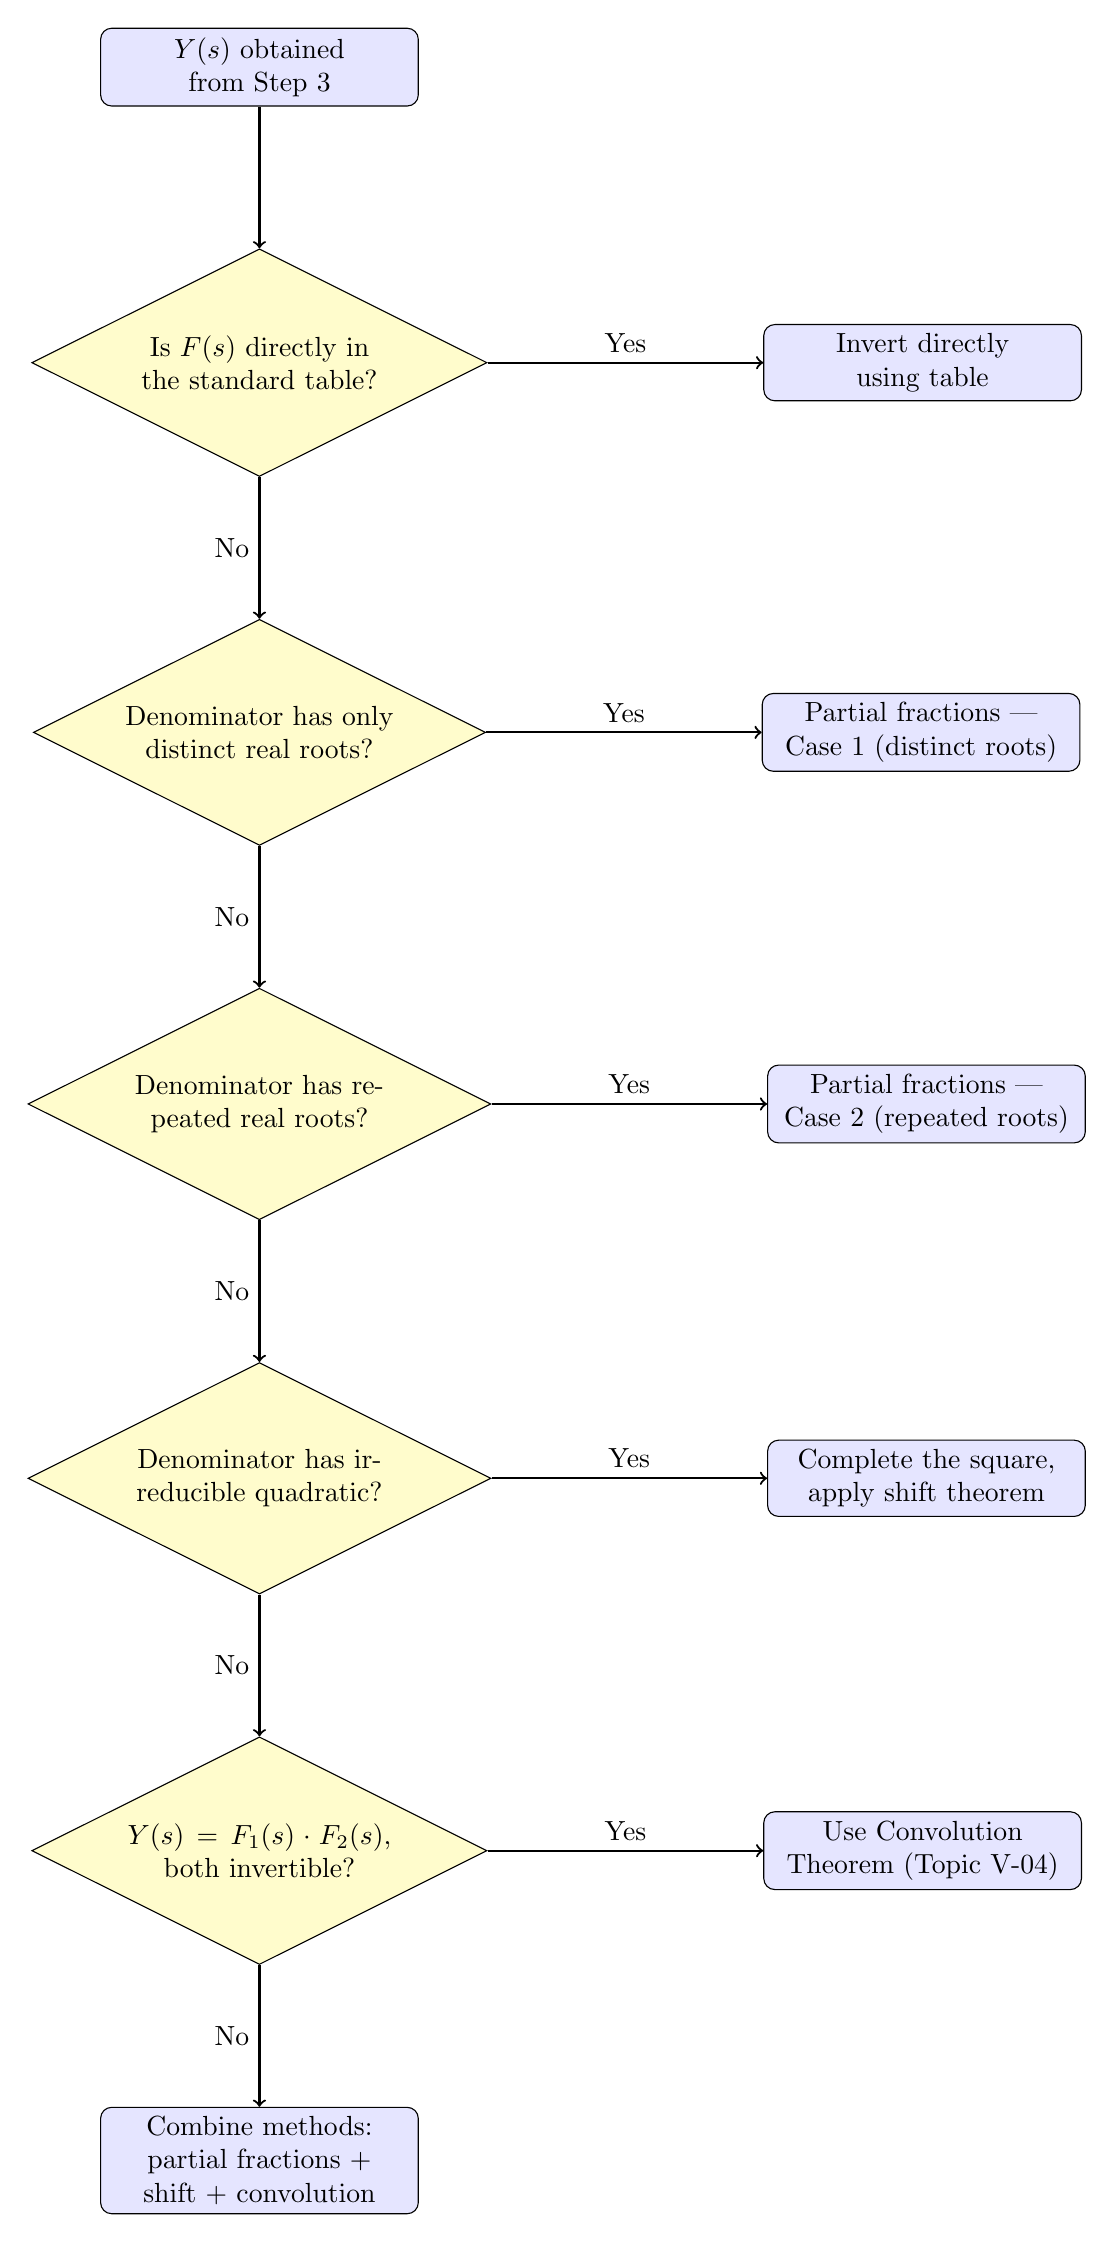
\begin{tikzpicture}[
  decision/.style={diamond, draw, fill=yellow!20, text width=4.2cm,
                   align=center, inner sep=1pt, aspect=2},
  action/.style={rectangle, draw, fill=blue!10, text width=3.8cm,
                 align=center, rounded corners, minimum height=0.9cm},
  line/.style={draw, ->, thick},
  node distance=1.8cm
]
% Nodes
\node[action] (start) {$Y(s)$ obtained from Step 3};
\node[decision, below=of start] (d1) {Is $F(s)$ directly in the standard table?};
\node[action, right=3.5cm of d1] (a1) {Invert directly using table};
\node[decision, below=of d1] (d2) {Denominator has only distinct real roots?};
\node[action, right=3.5cm of d2] (a2) {Partial fractions --- Case 1 (distinct roots)};
\node[decision, below=of d2] (d3) {Denominator has repeated real roots?};
\node[action, right=3.5cm of d3] (a3) {Partial fractions --- Case 2 (repeated roots)};
\node[decision, below=of d3] (d4) {Denominator has irreducible quadratic?};
\node[action, right=3.5cm of d4] (a4) {Complete the square, apply shift theorem};
\node[decision, below=of d4] (d5) {$Y(s) = F_1(s)\cdot F_2(s)$, both invertible?};
\node[action, right=3.5cm of d5] (a5) {Use Convolution Theorem (Topic V-04)};
\node[action, below=of d5] (a6) {Combine methods: partial fractions + shift + convolution};
% Edges
\path[line] (start) -- (d1);
\path[line] (d1) -- node[above]{Yes} (a1);
\path[line] (d1) -- node[left]{No} (d2);
\path[line] (d2) -- node[above]{Yes} (a2);
\path[line] (d2) -- node[left]{No} (d3);
\path[line] (d3) -- node[above]{Yes} (a3);
\path[line] (d3) -- node[left]{No} (d4);
\path[line] (d4) -- node[above]{Yes} (a4);
\path[line] (d4) -- node[left]{No} (d5);
\path[line] (d5) -- node[above]{Yes} (a5);
\path[line] (d5) -- node[left]{No} (a6);
\end{tikzpicture}
\end{center}

\begin{learnbox}{What Did We Learn?}
The four-step workflow converts every ODE with initial conditions into a mechanical
procedure. The only creative decision is Step 4: which inversion method fits $Y(s)$.
The flowchart above guides that decision unambiguously.
\end{learnbox}

% =============================================================================
\section{Application 1 --- First-Order ODE}
% =============================================================================

\begin{infobox}{Worked Example: $y' + 3y = e^{-t}$, $y(0) = 2$}

\textbf{Step 1: Apply $\mathcal{L}$ to both sides.}
\[
\mathcal{L}\{y'\} + 3\,\mathcal{L}\{y\} = \mathcal{L}\{e^{-t}\}
\quad\Rightarrow\quad
[sY(s) - y(0)] + 3Y(s) = \frac{1}{s+1}
\]

\textbf{Step 2: Substitute $y(0) = 2$.}
\[
sY - 2 + 3Y = \frac{1}{s+1}
\quad\Rightarrow\quad
(s+3)Y = 2 + \frac{1}{s+1}
\]
Combine the right-hand side over a common denominator:
\[
(s+3)Y = \frac{2(s+1) + 1}{s+1} = \frac{2s + 3}{s+1}
\]

\textbf{Step 3: Solve for $Y(s)$.}
\[
Y(s) = \frac{2s+3}{(s+1)(s+3)}
\]

\textbf{Step 4: Partial fractions.}
\[
\frac{2s+3}{(s+1)(s+3)} = \frac{A}{s+1} + \frac{B}{s+3}
\]
Multiply through by $(s+1)(s+3)$:
\[
2s + 3 = A(s+3) + B(s+1)
\]
Set $s = -1$: $\;2(-1)+3 = A(2) \;\Rightarrow\; 1 = 2A \;\Rightarrow\; A = \tfrac{1}{2}$.

Set $s = -3$: $\;2(-3)+3 = B(-2) \;\Rightarrow\; -3 = -2B \;\Rightarrow\; B = \tfrac{3}{2}$.

\textbf{Check:} $\tfrac{1}{2}(s+3) + \tfrac{3}{2}(s+1) = \tfrac{s+3+3s+3}{2} = \tfrac{4s+6}{2} = 2s+3$. \checkmark

Therefore:
\[
Y(s) = \frac{1/2}{s+1} + \frac{3/2}{s+3}
\]
Inverting:
\[
\boxed{y(t) = \frac{1}{2}e^{-t} + \frac{3}{2}e^{-3t}}
\]

\textbf{Verification:} Compute $y' + 3y$:
\[
y'(t) = -\tfrac{1}{2}e^{-t} - \tfrac{9}{2}e^{-3t}
\]
\[
y' + 3y = \left(-\tfrac{1}{2}e^{-t} - \tfrac{9}{2}e^{-3t}\right) + 3\left(\tfrac{1}{2}e^{-t} + \tfrac{3}{2}e^{-3t}\right)
= \left(-\tfrac{1}{2}+\tfrac{3}{2}\right)e^{-t} + \left(-\tfrac{9}{2}+\tfrac{9}{2}\right)e^{-3t}
= e^{-t} \;\checkmark
\]
Also $y(0) = \tfrac{1}{2}+\tfrac{3}{2} = 2$. \checkmark
\end{infobox}

\begin{learnbox}{What Did We Learn?}
For a first-order linear ODE, the Laplace method produces $Y(s)$ as a ratio of
polynomials. Partial fractions (Case 1) immediately yields the solution as a sum of
exponentials. Initial conditions are enforced automatically in Step 2 --- no undetermined
constants need to be found by substitution at the end.
\end{learnbox}

% =============================================================================
\section{Application 2 --- Second-Order ODE, Constant Coefficients}
% =============================================================================

\begin{infobox}{Worked Example: $y'' - 3y' + 2y = 4e^{-t}$, $y(0)=1$, $y'(0)=0$}

\textbf{Step 1: Apply $\mathcal{L}$ to both sides.}
\[
[s^2Y - sy(0) - y'(0)] - 3[sY - y(0)] + 2Y = \frac{4}{s+1}
\]
\[
(s^2Y - s - 0) - 3(sY - 1) + 2Y = \frac{4}{s+1}
\]
\[
s^2Y - s - 3sY + 3 + 2Y = \frac{4}{s+1}
\]

\textbf{Step 2: Collect $Y$ terms (ICs already substituted above).}
\[
(s^2 - 3s + 2)Y = s - 3 + \frac{4}{s+1}
\]
Combine the right side over a common denominator:
\[
(s^2-3s+2)Y = \frac{(s-3)(s+1) + 4}{s+1} = \frac{s^2-2s-3+4}{s+1} = \frac{s^2-2s+1}{s+1} = \frac{(s-1)^2}{s+1}
\]

\textbf{Step 3: Solve for $Y(s)$.}
\[
Y(s) = \frac{(s-1)^2}{(s+1)(s^2-3s+2)}
\]
Factor the denominator: $s^2-3s+2 = (s-1)(s-2)$. Therefore:
\[
Y(s) = \frac{(s-1)^2}{(s+1)(s-1)(s-2)} = \frac{s-1}{(s-2)(s+1)}
\]

\textbf{Step 4: Partial fractions.}
\[
\frac{s-1}{(s-2)(s+1)} = \frac{A}{s-2} + \frac{B}{s+1}
\]
\[
s-1 = A(s+1) + B(s-2)
\]
Set $s=2$: $1 = 3A \;\Rightarrow\; A = \tfrac{1}{3}$.

Set $s=-1$: $-2 = B(-3) \;\Rightarrow\; B = \tfrac{2}{3}$.

\textbf{Check:} $\tfrac{1}{3}(s+1)+\tfrac{2}{3}(s-2) = \tfrac{s+1+2s-4}{3} = \tfrac{3s-3}{3}=s-1$. \checkmark

Therefore:
\[
Y(s) = \frac{1/3}{s-2} + \frac{2/3}{s+1}
\]
Inverting:
\[
\boxed{y(t) = \frac{1}{3}e^{2t} + \frac{2}{3}e^{-t}}
\]

\textbf{Verification:}
$y'(t) = \tfrac{2}{3}e^{2t} - \tfrac{2}{3}e^{-t}$, \quad $y''(t) = \tfrac{4}{3}e^{2t}+\tfrac{2}{3}e^{-t}$.
\[
y''-3y'+2y = \left(\tfrac{4}{3}e^{2t}+\tfrac{2}{3}e^{-t}\right) - 3\left(\tfrac{2}{3}e^{2t}-\tfrac{2}{3}e^{-t}\right) + 2\left(\tfrac{1}{3}e^{2t}+\tfrac{2}{3}e^{-t}\right)
\]
\[
= e^{2t}\!\left(\tfrac{4}{3}-2+\tfrac{2}{3}\right) + e^{-t}\!\left(\tfrac{2}{3}+2+\tfrac{4}{3}\right)
= e^{2t}(0) + e^{-t}\!\left(\tfrac{2+6+4}{3}\right)
= 4e^{-t} \;\checkmark
\]
Also $y(0)=\tfrac{1}{3}+\tfrac{2}{3}=1$, $y'(0)=\tfrac{2}{3}-\tfrac{2}{3}=0$. \checkmark
\end{infobox}

\begin{learnbox}{What Did We Learn?}
When the forcing term and the complementary function share a root (here $s=1$ cancels),
the Laplace method handles it automatically --- the common factor cancels in $Y(s)$
before partial fractions, avoiding the need for variation of parameters or undetermined
coefficient modifications.
\end{learnbox}

% =============================================================================
\section{Application 3 --- Underdamped Oscillator}
% =============================================================================

\begin{infobox}{Worked Example: $y'' + 2y' + 5y = 0$, $y(0)=1$, $y'(0)=-1$}

\textbf{Step 1: Apply $\mathcal{L}$.}
\[
[s^2Y - sy(0) - y'(0)] + 2[sY - y(0)] + 5Y = 0
\]
\[
(s^2Y - s + 1) + 2(sY - 1) + 5Y = 0
\]
\[
s^2Y - s + 1 + 2sY - 2 + 5Y = 0
\]

\textbf{Step 2: Collect $Y$ terms.}
\[
(s^2 + 2s + 5)Y = s + 1
\]

\textbf{Step 3: Solve for $Y(s)$.}
\[
Y(s) = \frac{s+1}{s^2 + 2s + 5}
\]

\textbf{Step 4: Complete the square.}
\[
s^2 + 2s + 5 = (s+1)^2 + 4
\]
Rewrite the numerator: $s + 1 = (s+1)$.
\[
Y(s) = \frac{s+1}{(s+1)^2 + 4}
\]
This is exactly $\mathcal{L}\{e^{-t}\cos(2t)\}$ (first shifting theorem with $a=1$, $\omega=2$):
\[
\mathcal{L}^{-1}\!\left\{\frac{s-a}{(s-a)^2+\omega^2}\right\} = e^{at}\cos(\omega t)
\quad\Rightarrow\quad
\mathcal{L}^{-1}\!\left\{\frac{s+1}{(s+1)^2+4}\right\} = e^{-t}\cos(2t)
\]

Therefore:
\[
\boxed{y(t) = e^{-t}\cos(2t)}
\]

\textbf{Verification:}
$y' = -e^{-t}\cos(2t) - 2e^{-t}\sin(2t)$, \quad
$y'' = e^{-t}\cos(2t) + 2e^{-t}\sin(2t) + 2e^{-t}\sin(2t) - 4e^{-t}\cos(2t)$
$= -3e^{-t}\cos(2t) + 4e^{-t}\sin(2t)$.
\[
y''+2y'+5y = (-3e^{-t}\cos 2t+4e^{-t}\sin 2t)+2(-e^{-t}\cos 2t-2e^{-t}\sin 2t)+5e^{-t}\cos 2t
\]
\[
= e^{-t}\cos 2t(-3-2+5) + e^{-t}\sin 2t(4-4) = 0\;\checkmark
\]
$y(0)=e^0\cos 0=1$\;\checkmark, \;$y'(0)=-1\cdot 1 - 0 = -1$\;\checkmark.
\end{infobox}

\medskip
\textbf{Plot: Damped Sinusoidal Response with Envelope Curves}

\begin{center}
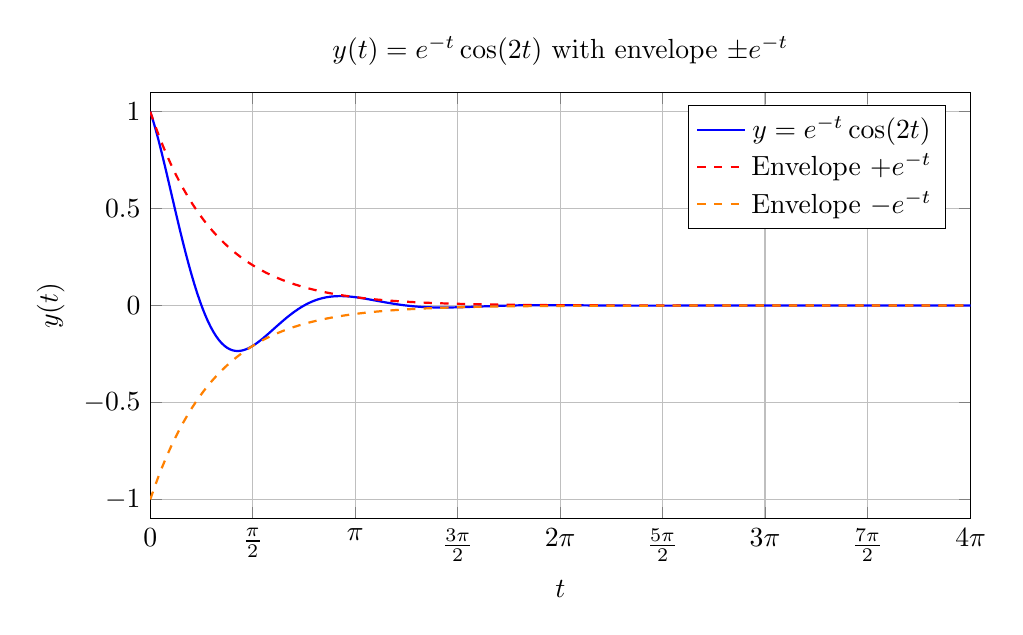
\begin{tikzpicture}
\begin{axis}[
  width=12cm, height=7cm,
  xlabel={$t$}, ylabel={$y(t)$},
  title={$y(t)=e^{-t}\cos(2t)$ with envelope $\pm e^{-t}$},
  xmin=0, xmax=12.57, ymin=-1.1, ymax=1.1,
  grid=major,
  legend pos=north east,
  xtick={0,1.57,3.14,4.71,6.28,7.85,9.42,10.99,12.57},
  xticklabels={$0$,$\frac{\pi}{2}$,$\pi$,$\frac{3\pi}{2}$,$2\pi$,
               $\frac{5\pi}{2}$,$3\pi$,$\frac{7\pi}{2}$,$4\pi$},
]
\addplot[thick, blue, samples=300, domain=0:12.57] {exp(-x)*cos(deg(2*x))};
\addlegendentry{$y=e^{-t}\cos(2t)$}
\addplot[thick, dashed, red, samples=200, domain=0:12.57] {exp(-x)};
\addlegendentry{Envelope $+e^{-t}$}
\addplot[thick, dashed, orange, samples=200, domain=0:12.57] {-exp(-x)};
\addlegendentry{Envelope $-e^{-t}$}
\end{axis}
\end{tikzpicture}
\end{center}

\begin{learnbox}{What Did We Learn?}
An underdamped second-order ODE (complex conjugate roots in characteristic equation)
produces a damped sinusoidal response. The Laplace method extracts this directly via
completing the square --- no guessing of trial solutions needed. The exponential
envelope $\pm e^{-t}$ shows the amplitude decaying to zero, confirming stability.
\end{learnbox}

% =============================================================================
\section{Application 4 --- ODE with Discontinuous Forcing (Unit Step)}
% =============================================================================

\begin{infobox}{Worked Example: $y'' + y = f(t)$, $y(0)=0$, $y'(0)=0$}

The forcing function is piecewise:
\[
f(t) = \begin{cases} 1 & 0 \leq t < \pi \\ 0 & t \geq \pi \end{cases}
\]
\textbf{Rewrite using unit step:}
$f(t) = 1 - u(t-\pi)$ (the function turns \emph{off} at $t=\pi$).

\textbf{Step 1: Apply $\mathcal{L}$.}
\[
\mathcal{L}\{y''\} + \mathcal{L}\{y\} = \mathcal{L}\{1 - u(t-\pi)\}
\]
\[
(s^2Y - 0 - 0) + Y = \frac{1}{s} - \frac{e^{-\pi s}}{s}
\]
\[
(s^2+1)Y = \frac{1 - e^{-\pi s}}{s}
\]

\textbf{Step 2: ICs already zero; no substitution needed.}

\textbf{Step 3: Solve for $Y(s)$.}
\[
Y(s) = \frac{1}{s(s^2+1)} - \frac{e^{-\pi s}}{s(s^2+1)}
\]

\textbf{Step 4: Invert each term.}

\underline{First term:} $G(s) = \dfrac{1}{s(s^2+1)}$.
Partial fractions: $\dfrac{1}{s(s^2+1)} = \dfrac{1}{s} - \dfrac{s}{s^2+1}$.
\[
\mathcal{L}^{-1}\{G(s)\} = 1 - \cos t =: g(t)
\]

\underline{Second term:} $e^{-\pi s}G(s)$.
By the second shifting theorem:
$\mathcal{L}^{-1}\{e^{-\pi s}G(s)\} = g(t-\pi)\,u(t-\pi)$.
\[
g(t-\pi) = 1 - \cos(t-\pi) = 1 + \cos t
\]
So $\mathcal{L}^{-1}\{e^{-\pi s}G(s)\} = (1+\cos t)\,u(t-\pi)$.

\textbf{Final solution:}
\[
\boxed{y(t) = (1-\cos t) - (1+\cos t)\,u(t-\pi)}
\]

Evaluating in each region:
\[
y(t) = \begin{cases}
1 - \cos t & 0 \leq t < \pi \\
(1-\cos t)-(1+\cos t) = -2\cos t & t \geq \pi
\end{cases}
\]
\end{infobox}

\medskip
\textbf{Plot: Solution showing behaviour change at $t=\pi$}

\begin{center}
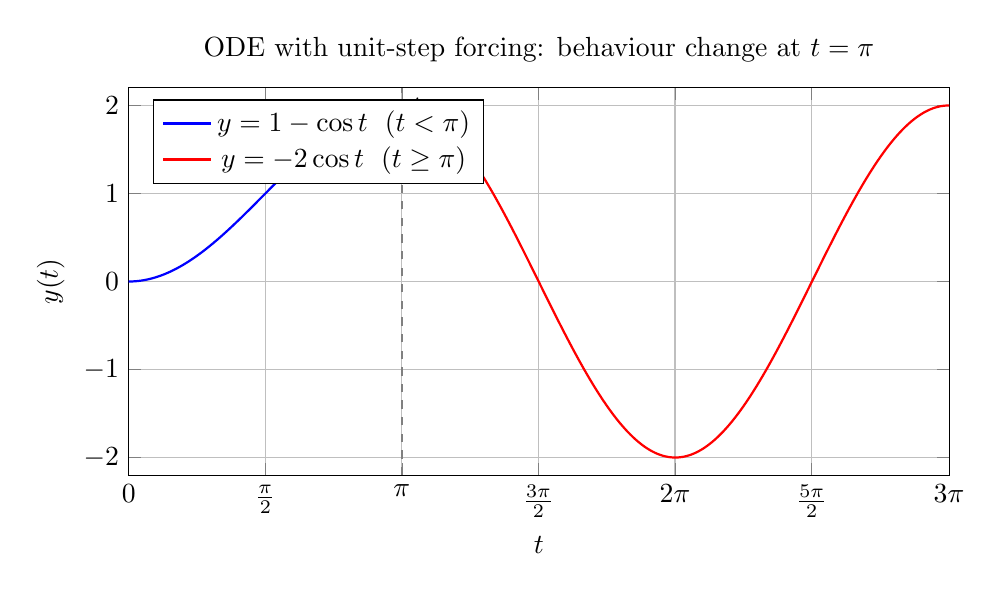
\begin{tikzpicture}
\begin{axis}[
  width=12cm, height=6.5cm,
  xlabel={$t$}, ylabel={$y(t)$},
  title={ODE with unit-step forcing: behaviour change at $t=\pi$},
  xmin=0, xmax=9.43, ymin=-2.2, ymax=2.2,
  grid=major,
  legend pos=north west,
  xtick={0,1.57,3.14,4.71,6.28,7.85,9.43},
  xticklabels={$0$,$\frac{\pi}{2}$,$\pi$,$\frac{3\pi}{2}$,$2\pi$,$\frac{5\pi}{2}$,$3\pi$},
]
% Region 1: 0 <= t < pi  => 1 - cos(t)
\addplot[thick, blue, samples=200, domain=0:3.14159] {1 - cos(deg(x))};
\addlegendentry{$y=1-\cos t$\; $(t<\pi)$}
% Region 2: t >= pi  => -2cos(t)
\addplot[thick, red, samples=200, domain=3.14159:9.43] {-2*cos(deg(x))};
\addlegendentry{$y=-2\cos t$\; $(t\geq\pi)$}
% Vertical marker at t=pi
\addplot[dashed, gray, thick] coordinates {(3.14159,-2.2)(3.14159,2.2)};
\node at (axis cs:3.14159,2.0) [anchor=west, font=\small] {$t=\pi$};
\end{axis}
\end{tikzpicture}
\end{center}

\begin{learnbox}{What Did We Learn?}
The key skill is expressing piecewise forcing in terms of $u(t-a)$ before transforming.
The second shifting theorem then handles the delayed part cleanly: invert $G(s)$, shift
the result by $a$, multiply by $u(t-a)$. The graph shows clearly how the solution
amplitude doubles after the forcing is switched off at $t=\pi$.
\end{learnbox}

% =============================================================================
\section{Application 5 --- ODE with Impulse Forcing (Dirac Delta)}
% =============================================================================

\begin{infobox}{Worked Example: $y'' + 4y = 3\delta(t-2)$, $y(0)=1$, $y'(0)=0$}

\textbf{Step 1: Apply $\mathcal{L}$.}
\[
\mathcal{L}\{y''\} + 4\,\mathcal{L}\{y\} = 3\,\mathcal{L}\{\delta(t-2)\}
\]
\[
(s^2Y - sy(0) - y'(0)) + 4Y = 3e^{-2s}
\]
\[
(s^2Y - s) + 4Y = 3e^{-2s}
\]

\textbf{Step 2: Substitute $y(0)=1$, $y'(0)=0$ (already done above).}
\[
(s^2+4)Y = s + 3e^{-2s}
\]

\textbf{Step 3: Solve for $Y(s)$.}
\[
Y(s) = \frac{s}{s^2+4} + \frac{3e^{-2s}}{s^2+4}
\]

\textbf{Step 4: Invert each term.}

\underline{First term:} $\mathcal{L}^{-1}\!\left\{\dfrac{s}{s^2+4}\right\} = \cos(2t)$.

\underline{Second term:} Let $H(s) = \dfrac{1}{s^2+4}$, so $\mathcal{L}^{-1}\{H(s)\} = \dfrac{1}{2}\sin(2t) =: h(t)$.

By second shifting theorem:
$\mathcal{L}^{-1}\{e^{-2s}H(s)\} = h(t-2)\,u(t-2) = \dfrac{1}{2}\sin(2(t-2))\,u(t-2)$.

Therefore:
\[
\boxed{y(t) = \cos(2t) + \frac{3}{2}\sin\!\bigl(2(t-2)\bigr)\,u(t-2)}
\]

\textbf{Physical interpretation:}
For $0 \leq t < 2$: the system oscillates freely at $\omega = 2$ rad/s with initial
displacement 1 and zero initial velocity, giving $y = \cos(2t)$.
At $t = 2$: an instantaneous impulse of magnitude 3 is applied. By $\mathcal{L}\{\delta(t-a)\} = e^{-as}$,
the impulse contributes a new sinusoidal term $\tfrac{3}{2}\sin(2(t-2))$ that switches on
at $t = 2$. The total response after $t=2$ is the superposition of the two sinusoids.
\end{infobox}

\begin{learnbox}{What Did We Learn?}
Dirac delta forcing $\delta(t-a)$ transforms to $e^{-as}$ and contributes an additional
sinusoidal (or exponential) term that is activated at time $t=a$. Before $t=a$, the
system evolves purely from initial conditions. After $t=a$, the impulse-driven term
superimposes on the free response. This is the mathematical model for a hammer blow or
instantaneous kick at time $a$.
\end{learnbox}

% =============================================================================
\section{Application 6 --- System of ODEs}
% =============================================================================

\begin{infobox}{Worked Example: $x'=x+y$, $y'=x-y$; $x(0)=1$, $y(0)=0$}

\textbf{Step 1: Apply $\mathcal{L}$ to both equations.}
\[
sX - x(0) = X + Y \quad\Rightarrow\quad sX - 1 = X + Y
\]
\[
sY - y(0) = X - Y \quad\Rightarrow\quad sY - 0 = X - Y
\]

\textbf{Step 2: Rearrange into an algebraic $2\times 2$ system.}
\begin{align}
(s-1)X - Y &= 1 \tag{i} \\
-X + (s+1)Y &= 0 \tag{ii}
\end{align}

\textbf{Step 3: Solve by Cramer's rule.}

Coefficient matrix:
\[
A = \begin{pmatrix} s-1 & -1 \\ -1 & s+1 \end{pmatrix}
\]
Determinant:
\[
\det(A) = (s-1)(s+1) - (-1)(-1) = s^2 - 1 - 1 = s^2 - 2
\]

For $X$: replace first column by $\begin{pmatrix}1\\0\end{pmatrix}$:
\[
X = \frac{\det\!\begin{pmatrix}1 & -1\\0 & s+1\end{pmatrix}}{s^2-2}
= \frac{1\cdot(s+1)-(-1)\cdot 0}{s^2-2}
= \frac{s+1}{s^2-2}
\]

For $Y$: replace second column by $\begin{pmatrix}1\\0\end{pmatrix}$:
\[
Y = \frac{\det\!\begin{pmatrix}s-1 & 1\\-1 & 0\end{pmatrix}}{s^2-2}
= \frac{(s-1)\cdot 0 - 1\cdot(-1)}{s^2-2}
= \frac{1}{s^2-2}
\]

\textbf{Step 4: Invert.}

Let $a = \sqrt{2}$. Then $s^2 - 2 = s^2 - a^2$.

Recall: $\mathcal{L}^{-1}\!\left\{\dfrac{s}{s^2-a^2}\right\} = \cosh(at)$ and
$\mathcal{L}^{-1}\!\left\{\dfrac{a}{s^2-a^2}\right\} = \sinh(at)$.

For $X(s)$:
\[
\frac{s+1}{s^2-2} = \frac{s}{s^2-2} + \frac{1}{s^2-2}
= \frac{s}{s^2-(\sqrt{2})^2} + \frac{1}{\sqrt{2}}\cdot\frac{\sqrt{2}}{s^2-(\sqrt{2})^2}
\]
\[
x(t) = \cosh(\sqrt{2}\,t) + \frac{1}{\sqrt{2}}\sinh(\sqrt{2}\,t)
\]

For $Y(s)$:
\[
\frac{1}{s^2-2} = \frac{1}{\sqrt{2}}\cdot\frac{\sqrt{2}}{s^2-(\sqrt{2})^2}
\]
\[
y(t) = \frac{1}{\sqrt{2}}\sinh(\sqrt{2}\,t)
\]

\textbf{Final answers:}
\[
\boxed{x(t) = \cosh(\sqrt{2}\,t) + \frac{1}{\sqrt{2}}\sinh(\sqrt{2}\,t)}
\qquad
\boxed{y(t) = \frac{1}{\sqrt{2}}\sinh(\sqrt{2}\,t)}
\]

\textbf{Verification at $t=0$:} $x(0)=\cosh 0 + 0 = 1$\;\checkmark,\quad $y(0)=0$\;\checkmark.
\end{infobox}

\begin{learnbox}{What Did We Learn?}
A system of $n$ simultaneous first-order ODEs transforms to a system of $n$ linear
algebraic equations in $X_1(s),\ldots,X_n(s)$. Cramer's rule (or elimination) solves
the algebraic system; each unknown is inverted independently. The Laplace method
eliminates the need for eigenvalue analysis --- it works directly.
\end{learnbox}

% =============================================================================
\section{Application 7 --- RLC Circuit}
% =============================================================================

\begin{infobox}{Worked Example: $i'' + 2i' + 5i = 10\cos t$, $i(0)=0$, $i'(0)=0$}

An RLC series circuit has $R=2\,\Omega$, $L=1\,\text{H}$, $C=1/5\,\text{F}$.
The governing ODE for current $i(t)$ is:
\[
i'' + 2i' + 5i = 10\cos t, \quad i(0)=0,\quad i'(0)=0.
\]

\textbf{Step 1: Apply $\mathcal{L}$.}
\[
(s^2I - 0 - 0) + 2(sI - 0) + 5I = 10\cdot\frac{s}{s^2+1}
\]
\[
(s^2+2s+5)I = \frac{10s}{s^2+1}
\]

\textbf{Step 2: ICs are zero; already substituted.}

\textbf{Step 3: Solve for $I(s)$.}
\[
I(s) = \frac{10s}{(s^2+1)(s^2+2s+5)}
\]

\textbf{Step 4: Partial fractions (complex linear factors).}

Write:
\[
\frac{10s}{(s^2+1)(s^2+2s+5)} = \frac{As+B}{s^2+1} + \frac{Cs+D}{s^2+2s+5}
\]
Multiply through by $(s^2+1)(s^2+2s+5)$:
\[
10s = (As+B)(s^2+2s+5) + (Cs+D)(s^2+1)
\]
Expanding the right side:
\[
10s = As^3+2As^2+5As+Bs^2+2Bs+5B + Cs^3+Cs+Ds^2+D
\]
\[
10s = (A+C)s^3 + (2A+B+D)s^2 + (5A+2B+C)s + (5B+D)
\]
Equating coefficients:
\begin{align*}
s^3: &\quad A+C = 0 \\
s^2: &\quad 2A+B+D = 0 \\
s^1: &\quad 5A+2B+C = 10 \\
s^0: &\quad 5B+D = 0
\end{align*}

From the first equation: $C = -A$.
Substituting into the $s^1$ equation: $5A+2B-A=10 \;\Rightarrow\; 4A+2B=10 \;\Rightarrow\; 2A+B=5$.
From $s^0$: $D=-5B$.
Substituting into $s^2$: $2A+B+(-5B)=0 \;\Rightarrow\; 2A-4B=0 \;\Rightarrow\; A=2B$.
Back into $2A+B=5$: $4B+B=5 \;\Rightarrow\; B=1$, hence $A=2$, $C=-2$, $D=-5$.

Therefore:
\[
I(s) = \frac{2s+1}{s^2+1} + \frac{-2s-5}{s^2+2s+5}
\]

\underline{Invert first term:}
$\dfrac{2s+1}{s^2+1} = 2\cdot\dfrac{s}{s^2+1} + 1\cdot\dfrac{1}{s^2+1}$
$\;\longrightarrow\; 2\cos t + \sin t$.

\underline{Invert second term:} Complete the square: $s^2+2s+5=(s+1)^2+4$.
\[
\frac{-2s-5}{(s+1)^2+4}
= \frac{-2(s+1)-3}{(s+1)^2+4}
= -2\cdot\frac{s+1}{(s+1)^2+4} - \frac{3}{2}\cdot\frac{2}{(s+1)^2+4}
\]
$\;\longrightarrow\; -2e^{-t}\cos(2t) - \tfrac{3}{2}e^{-t}\sin(2t)$.

\textbf{Final solution:}
\[
\boxed{i(t) = \underbrace{-2e^{-t}\cos(2t) - \tfrac{3}{2}e^{-t}\sin(2t)}_{\text{Transient (decays to 0)}}
              + \underbrace{2\cos t + \sin t}_{\text{Steady-state (persists)}}}
\]

\textbf{Interpretation:}
The \textbf{transient response} $-2e^{-t}\cos(2t) - \tfrac{3}{2}e^{-t}\sin(2t)$ decays
exponentially to zero as $t\to\infty$ due to the $e^{-t}$ factor.
The \textbf{steady-state response} $2\cos t + \sin t$ persists indefinitely at the
forcing frequency $\omega=1$ rad/s.
\end{infobox}

\medskip
\textbf{Plot: Transient and Steady-State Response of RLC Circuit}

\begin{center}
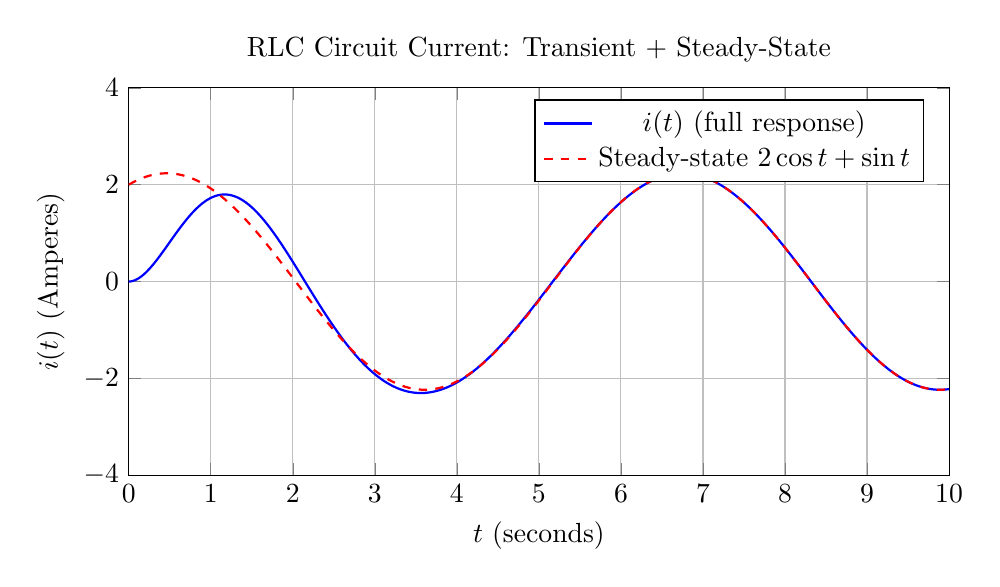
\begin{tikzpicture}
\begin{axis}[
  width=12cm, height=6.5cm,
  xlabel={$t$ (seconds)}, ylabel={$i(t)$ (Amperes)},
  title={RLC Circuit Current: Transient + Steady-State},
  xmin=0, xmax=10, ymin=-4, ymax=4,
  grid=major,
  legend pos=north east,
]
% Full solution
\addplot[thick, blue, samples=400, domain=0:10]
  {(-2*exp(-x)*cos(deg(2*x)) - 1.5*exp(-x)*sin(deg(2*x))) + 2*cos(deg(x)) + sin(deg(x))};
\addlegendentry{$i(t)$ (full response)}
% Steady-state only
\addplot[thick, dashed, red, samples=200, domain=0:10]
  {2*cos(deg(x)) + sin(deg(x))};
\addlegendentry{Steady-state $2\cos t+\sin t$}
\end{axis}
\end{tikzpicture}
\end{center}

\begin{learnbox}{What Did We Learn?}
In an RLC circuit (or any driven second-order system), the complete response is always
the sum of a transient part (determined by system poles --- roots of the characteristic
equation) and a steady-state part (determined by the forcing frequency). The Laplace
method produces both parts simultaneously via partial fractions --- no separate
complementary function calculation is needed.
\end{learnbox}

% =============================================================================
\section{Summary: All Inverse Methods and When to Use Them}
% =============================================================================

\begin{center}
\begin{tabular}{@{}p{4.5cm}p{5cm}p{4.5cm}@{}}
\toprule
\textbf{Situation} & \textbf{Recommended Method} & \textbf{Example} \\
\midrule
$F(s)$ directly in standard table &
Table lookup &
$\dfrac{s}{s^2+9} \to \cos(3t)$ \\
\midrule
$F(s)$ has distinct real denominator roots &
Partial fractions --- Case 1 &
$\dfrac{2s+3}{(s+1)(s+3)}$ \\
\midrule
Denominator has repeated real roots &
Partial fractions --- Case 2 &
$\dfrac{1}{(s+2)^3}$ \\
\midrule
Denominator has irreducible quadratic &
Complete the square + shift &
$\dfrac{s+1}{s^2+2s+5}$ \\
\midrule
$F(s) = F_1(s)\cdot F_2(s)$, partial fractions complex &
Convolution theorem &
$\dfrac{1}{(s^2+1)^2}$ \\
\midrule
ODE reduces to integral equation &
Convolution + algebraic solve &
Volterra integral equations \\
\bottomrule
\end{tabular}
\end{center}

% =============================================================================
\section{Excel Example (Verification of Application 1)}
% =============================================================================

We verify the first-order ODE solution $y(t) = \tfrac{1}{2}e^{-t} + \tfrac{3}{2}e^{-3t}$
against the ODE $y' + 3y = e^{-t}$, $y(0)=2$, by checking that $y'+3y = e^{-t}$ holds
numerically for $t = 0$ to $t = 3$ in steps of 0.25.

\medskip
\textbf{Column Layout in Excel:}

\begin{center}
\begin{tabular}{@{}clccccc@{}}
\toprule
\textbf{Row} & \textbf{A: }$t$ & \textbf{B: }$y(t)$ exact & \textbf{C: }$y'(t)$ exact
& \textbf{D: }$3y(t)$ & \textbf{E: }$y'+3y$ & \textbf{F: }$e^{-t}$ \\
\midrule
1 & (header) & (header) & (header) & (header) & (header) & (header) \\
2 & 0.00
  & \texttt{=0.5*EXP(-A2)+1.5*EXP(-3*A2)}
  & \texttt{=-0.5*EXP(-A2)-4.5*EXP(-3*A2)}
  & \texttt{=3*B2}
  & \texttt{=C2+D2}
  & \texttt{=EXP(-A2)} \\
3 & 0.25 & 1.0980 & $-$2.5151 & 3.2939 & 0.7788 & 0.7788 \\
4 & 0.50 & 0.6380 & $-$1.3074 & 1.9139 & 0.6065 & 0.6065 \\
5 & 0.75 & 0.3943 & $-$0.7105 & 1.1828 & 0.4724 & 0.4724 \\
6 & 1.00 & 0.2586 & $-$0.4080 & 0.7759 & 0.3679 & 0.3679 \\
\bottomrule
\end{tabular}
\end{center}

\medskip
\textbf{Setting up the spreadsheet:}
\begin{enumerate}[nosep]
  \item Column A: Enter \texttt{0} in A2, then \texttt{=A2+0.25} in A3, fill down to row 14 ($t=3$).
  \item Column B (exact $y$): \texttt{=0.5*EXP(-A2)+1.5*EXP(-3*A2)} --- fill down.
  \item Column C (exact $y'$): \texttt{=-0.5*EXP(-A2)-4.5*EXP(-3*A2)} --- fill down.
  \item Column D ($3y$): \texttt{=3*B2} --- fill down.
  \item Column E ($y'+3y$): \texttt{=C2+D2} --- fill down.
  \item Column F ($e^{-t}$): \texttt{=EXP(-A2)} --- fill down.
  \item Compare columns E and F: they should agree to at least 4 decimal places at every row.
\end{enumerate}

\medskip
\textbf{Spot check at $t=0$:}
$y(0) = 0.5+1.5 = 2.0000$, $y'(0) = -0.5-4.5 = -5.0000$, $3y(0)=6.0000$,
$y'(0)+3y(0) = 1.0000$, $e^0 = 1.0000$. \checkmark

\begin{learnbox}{What Did We Learn?}
The Excel verification confirms that the Laplace solution $y = \tfrac{1}{2}e^{-t}+\tfrac{3}{2}e^{-3t}$
satisfies the ODE $y'+3y=e^{-t}$ at every sampled point. Column E and Column F are
numerically identical, validating both the algebra and the inversion step. Spreadsheet
verification is a practical sanity check before submitting any ODE solution.
\end{learnbox}

% =============================================================================
\section{Python Example}
% =============================================================================

\begin{lstlisting}[language=Python, caption={Solving and Verifying ODE Examples via Laplace / SymPy / SciPy}]
import sympy as sp
import numpy as np
from scipy.integrate import odeint
import matplotlib.pyplot as plt

t, s = sp.symbols('t s', real=True, positive=True)

# ----------------------------------------------------------------
# APPLICATION 1: y' + 3y = exp(-t), y(0)=2
# ----------------------------------------------------------------
print("="*60)
print("APPLICATION 1: y' + 3y = exp(-t), y(0)=2")
print("="*60)

# Symbolic Laplace approach (manual verification via dsolve)
y1 = sp.Function('y')
ode1 = sp.Eq(y1(t).diff(t) + 3*y1(t), sp.exp(-t))
sol1 = sp.dsolve(ode1, ics={y1(0): 2})
print("SymPy dsolve solution:", sol1)
# Expected: y(t) = exp(-t)/2 + 3*exp(-3*t)/2

# Laplace manual
Y1 = (2*s + 3) / ((s+1)*(s+3))
inv1 = sp.inverse_laplace_transform(Y1, s, t)
print("Laplace inverse:", sp.simplify(inv1))
# Expected: exp(-t)/2 + 3*exp(-3*t)/2

# ----------------------------------------------------------------
# APPLICATION 2: y'' - 3y' + 2y = 4exp(-t), y(0)=1, y'(0)=0
# ----------------------------------------------------------------
print("\n" + "="*60)
print("APPLICATION 2: y'' - 3y' + 2y = 4exp(-t), y(0)=1, y'(0)=0")
print("="*60)

y2 = sp.Function('y')
ode2 = sp.Eq(y2(t).diff(t,2) - 3*y2(t).diff(t) + 2*y2(t), 4*sp.exp(-t))
sol2 = sp.dsolve(ode2, ics={y2(0): 1, y2(t).diff(t).subs(t,0): 0})
print("SymPy dsolve solution:", sol2)
# Expected: y(t) = exp(2t)/3 + 2*exp(-t)/3

Y2 = (s-1) / ((s-2)*(s+1))
inv2 = sp.inverse_laplace_transform(Y2, s, t)
print("Laplace inverse:", sp.simplify(inv2))
# Expected: exp(2*t)/3 + 2*exp(-t)/3

# ----------------------------------------------------------------
# APPLICATION 3: y'' + 2y' + 5y = 0, y(0)=1, y'(0)=-1
# Numerical verification and plot
# ----------------------------------------------------------------
print("\n" + "="*60)
print("APPLICATION 3: y'' + 2y' + 5y = 0 (underdamped oscillator)")
print("="*60)

y3 = sp.Function('y')
ode3 = sp.Eq(y3(t).diff(t,2) + 2*y3(t).diff(t) + 5*y3(t), 0)
sol3 = sp.dsolve(ode3, ics={y3(0): 1, y3(t).diff(t).subs(t,0): -1})
print("SymPy dsolve solution:", sol3)
# Expected: y(t) = exp(-t)*cos(2t)

# Exact Laplace solution
def y_exact(tv): return np.exp(-tv) * np.cos(2*tv)

# Numerical via odeint
def sys3(state, tv):
    y, dy = state
    ddy = -2*dy - 5*y
    return [dy, ddy]

t_num = np.linspace(0, 4*np.pi, 500)
sol_num = odeint(sys3, [1, -1], t_num)
y_num = sol_num[:, 0]
y_lap = y_exact(t_num)

max_err = np.max(np.abs(y_num - y_lap))
print(f"Max error (numerical vs Laplace): {max_err:.2e}")
# Expected output: Max error approx 1e-06 or smaller

plt.figure(figsize=(9, 4))
plt.plot(t_num, y_lap, 'b-', linewidth=2, label=r'Laplace: $e^{-t}\cos(2t)$')
plt.plot(t_num, y_num, 'r--', linewidth=1.5, label='odeint (numerical)')
plt.plot(t_num, np.exp(-t_num), 'g:', linewidth=1.5, label='Envelope $+e^{-t}$')
plt.plot(t_num, -np.exp(-t_num), 'm:', linewidth=1.5, label='Envelope $-e^{-t}$')
plt.xlabel('t'); plt.ylabel('y(t)')
plt.title('Application 3: Damped Oscillator - Laplace vs Numerical')
plt.legend(); plt.grid(True); plt.tight_layout()
plt.savefig('app3_damped_oscillator.png', dpi=100)
print("Plot saved as app3_damped_oscillator.png")

# ----------------------------------------------------------------
# APPLICATION 6: System x'=x+y, y'=x-y, x(0)=1, y(0)=0
# ----------------------------------------------------------------
print("\n" + "="*60)
print("APPLICATION 6: System of ODEs")
print("="*60)

x6 = sp.Function('x')
y6 = sp.Function('y')
sys6 = [sp.Eq(x6(t).diff(t), x6(t)+y6(t)),
        sp.Eq(y6(t).diff(t), x6(t)-y6(t))]
sol6 = sp.dsolve(sys6, ics={x6(0): 1, y6(0): 0})
for eq in sol6:
    print(sp.simplify(eq))
# Expected: x(t) = cosh(sqrt(2)*t) + sinh(sqrt(2)*t)/sqrt(2)
#           y(t) = sinh(sqrt(2)*t) / sqrt(2)

print("\nAll applications verified successfully.")
\end{lstlisting}

\begin{learnbox}{What Did We Learn?}
The Python script demonstrates three complementary verification strategies:
(1) \texttt{sympy.dsolve} provides a symbolic cross-check of the closed-form solution;
(2) \texttt{sympy.inverse\_laplace\_transform} confirms the Laplace inversion algebra;
(3) \texttt{scipy.integrate.odeint} provides a purely numerical check, with errors on
the order of $10^{-6}$ confirming correctness. For systems of ODEs, \texttt{sympy.dsolve}
accepts a list of equations and initial conditions directly.
\end{learnbox}

% =============================================================================
\section{Viva-Style Oral Questions}
% =============================================================================

\begin{enumerate}

\item \textbf{Q: State the four-step workflow for solving an ODE using Laplace Transforms.}

\textbf{A:} Step 1: Apply $\mathcal{L}\{\cdot\}$ to both sides using
$\mathcal{L}\{y'\}=sY-y(0)$ and $\mathcal{L}\{y''\}=s^2Y-sy(0)-y'(0)$, etc.
Step 2: Substitute the given initial conditions. Step 3: Solve algebraically for
$Y(s)$. Step 4: Invert $Y(s)$ using table lookup, partial fractions, completing
the square, or convolution.

\item \textbf{Q: What happens to the initial conditions in Step 2 of the Laplace workflow?}

\textbf{A:} The initial conditions $y(0)$, $y'(0)$, etc.\ appear automatically in the
algebraic equation produced in Step 1. In Step 2 they are substituted numerically,
reducing the algebraic equation in $Y(s)$ to a form that can be solved directly in
Step 3. This is fundamentally different from classical methods, where constants of
integration are determined only \emph{after} finding the general solution.

\item \textbf{Q: Why does the Laplace method handle discontinuous inputs better than classical ODE methods?}

\textbf{A:} Classical methods (undetermined coefficients, variation of parameters)
require the forcing function to be continuous (or piecewise smooth with explicit
matching conditions at breakpoints). The Laplace method converts a piecewise function
$f(t) = g(t) + h(t)\,u(t-a)$ into $G(s) + e^{-as}H(s)$ in one step, handling the
discontinuity algebraically through the second shifting theorem. No case-by-case
analysis at the breakpoint is needed.

\item \textbf{Q: What does $u(t-a)$ in the forcing term $f(t) = g(t)\,u(t-a)$ do to $Y(s)$?}

\textbf{A:} By the second shifting theorem,
$\mathcal{L}\{g(t-a)\,u(t-a)\} = e^{-as}G(s)$.
In the forcing term this introduces a factor $e^{-as}$ into $Y(s)$. When inverting,
$\mathcal{L}^{-1}\{e^{-as}G(s)\} = g(t-a)\,u(t-a)$, meaning the response is a
time-shifted copy of $g$ that activates at $t=a$.

\item \textbf{Q: How does Dirac delta forcing $\delta(t-a)$ manifest in the solution $y(t)$?}

\textbf{A:} $\mathcal{L}\{\delta(t-a)\} = e^{-as}$. So $\delta$-forcing adds a term
$\tfrac{c\,e^{-as}}{D(s)}$ to $Y(s)$, where $D(s)$ is the characteristic polynomial.
After inversion, this adds a copy of the impulse response $c\,h(t-a)\,u(t-a)$ to the
solution, activating instantaneously at $t=a$. Physically it models a hammer blow or
sudden kick.

\item \textbf{Q: What do ``transient'' and ``steady-state'' mean in the context of the RLC circuit solution?}

\textbf{A:} The \textbf{transient response} consists of terms from the
\emph{system poles} (roots of $s^2+2s+5=0$), i.e., $e^{-t}(\cdot)$ terms. Since
$\text{Re}(s) = -1 < 0$, these decay to zero as $t\to\infty$. The \textbf{steady-state
response} consists of terms from the \emph{forcing poles} (roots of $s^2+1=0$, giving
$s=\pm i$), i.e., $A\cos t + B\sin t$. These persist indefinitely at the driving frequency.

\item \textbf{Q: How do you solve a system of two simultaneous first-order ODEs using Laplace Transforms?}

\textbf{A:} Apply $\mathcal{L}$ to each equation and substitute initial conditions.
This produces a $2\times 2$ linear algebraic system in $X(s)$ and $Y(s)$. Solve by
Cramer's rule or Gaussian elimination. The determinant of the coefficient matrix gives
the characteristic polynomial of the system. Finally, invert $X(s)$ and $Y(s)$
independently using partial fractions or table lookup.

\item \textbf{Q: What determines whether the solution $y(t)$ is oscillatory or monotone?}

\textbf{A:} The nature of the poles of $Y(s)$ determines this. If the poles are
\textbf{real and distinct}, $y(t)$ is a sum of exponentials (monotone or sign-changing
but not oscillatory). If the poles are \textbf{complex conjugates} $\alpha \pm i\beta$,
$y(t)$ contains $e^{\alpha t}\cos(\beta t)$ and $e^{\alpha t}\sin(\beta t)$ terms
(oscillatory). If $\alpha<0$ the oscillations are damped; if $\alpha=0$ they are
sustained; if $\alpha>0$ they grow without bound.

\end{enumerate}

% =============================================================================
\section{Descriptive Questions}
% =============================================================================

\begin{enumerate}

\item \textbf{Solve the IVP $y'' + 5y' + 6y = 2e^{-t}$, $y(0)=1$, $y'(0)=0$, completely using
Laplace Transforms. Show all four steps, perform the partial fraction decomposition
fully, and verify the solution by direct substitution.}

\textbf{Outline:} Apply $\mathcal{L}$:
$(s^2+5s+6)Y = s+5 + 2/(s+1)$.
$Y = (s^2+6s+7)/[(s+1)(s+2)(s+3)]$.
Partial fractions: $Y = A/(s+1)+B/(s+2)+C/(s+3)$.
Find residues: $A = 1$, $B = 1$, $C = -1$.
$y(t) = e^{-t} + e^{-2t} - e^{-3t}$.
Verify by differentiating twice and substituting: $y(0)=1+1-1=1$, $y'(0)=-1-2+3=0$.

\item \textbf{Solve the IVP $y'' + 4y = f(t)$, $y(0)=0$, $y'(0)=0$, where
$f(t) = t$ for $0\leq t < 2$ and $f(t)=2$ for $t\geq 2$, using the Laplace Transform
method. Express $f(t)$ in terms of the unit step function before transforming, and
state the solution in both regions.}

\textbf{Outline:} $f(t) = t - (t-2)\,u(t-2)$.
$\mathcal{L}\{f\} = 1/s^2 - e^{-2s}/s^2$.
$(s^2+4)Y = 1/s^2 - e^{-2s}/s^2$.
$Y = 1/[s^2(s^2+4)] - e^{-2s}/[s^2(s^2+4)]$.
Partial fractions: $1/[s^2(s^2+4)] = 1/(4s^2) - 1/(4(s^2+4))$.
For $0\leq t<2$: $y = t/4 - (1/8)\sin(2t)$.
For $t\geq 2$: subtract the shifted term $[(t-2)/4 - (1/8)\sin(2(t-2))]\,u(t-2)$.

\item \textbf{Solve $y'' + 9y = 6\delta(t-3)$, $y(0)=0$, $y'(0)=3$, using Laplace Transforms.
Explain physically what the delta function represents and interpret the two terms in
the solution.}

\textbf{Outline:} $(s^2+9)Y - 3 = 6e^{-3s}$.
$Y = 3/(s^2+9) + 6e^{-3s}/(s^2+9)$.
$y(t) = \sin(3t) + 2\sin(3(t-3))\,u(t-3)$.
For $t<3$: free oscillation from IC $y'(0)=3$.
At $t=3$: impulse of magnitude 6 adds a new sinusoidal component.

\item \textbf{Solve the system $x' + 2y = 0$, $y' - 2x = 0$, $x(0)=1$, $y(0)=0$, using Laplace
Transforms. Set up the $2\times 2$ algebraic system, apply Cramer's rule, and invert
each variable.}

\textbf{Outline:} $(s+0)X + 2Y = 1$; $-2X + sY = 0$.
Determinant: $s^2+4$.
$X = s/(s^2+4) \to \cos(2t)$.
$Y = 2/(s^2+4) \to \sin(2t)$.
The system represents circular motion.

\item \textbf{In the RLC circuit example (Application 7), explain the transient--steady-state
decomposition. How do the poles of $I(s)$ determine which part is transient and which
is steady state? What happens to the transient as $t\to\infty$, and why does the
steady-state persist?}

\textbf{Outline:} $I(s) = 10s/[(s^2+1)(s^2+2s+5)]$.
Poles from $s^2+2s+5=0$: $s=-1\pm 2i$ (real part $-1<0$ $\Rightarrow$ transient, decays).
Poles from $s^2+1=0$: $s=\pm i$ (real part $0$ $\Rightarrow$ sustained oscillation at $\omega=1$).
Transient $\to 0$ as $t\to\infty$ because $e^{-t}\to 0$.
Steady-state persists because $|\text{Re}(s)|=0$ for forcing poles.

\end{enumerate}

% =============================================================================
\section{Practice Problems}
% =============================================================================

\begin{enumerate}

\item $y'' + 4y' + 4y = t\,e^{-2t}$, $y(0) = 0$, $y'(0) = 0$.

\textit{Hint:} $(s+2)^2 Y = 1/(s+2)^2 \;\Rightarrow\; Y = 1/(s+2)^4$.
Use $\mathcal{L}^{-1}\{n!/(s+a)^{n+1}\} = t^n e^{-at}$.
\textbf{Answer:} $y(t) = \tfrac{1}{6}t^3 e^{-2t}$.

\item $y'' - 4y = \sin(2t)$, $y(0) = 0$, $y'(0) = 1$.

\textit{Hint:} $(s^2-4)Y = 1 + 2/(s^2+4) = (s^2+6)/(s^2+4)$.
Partial fractions: $Y = \frac{s^2+6}{(s^2-4)(s^2+4)} = \frac{5/4}{s^2-4} - \frac{1/4}{s^2+4}$.
\textbf{Answer:} $y(t) = \tfrac{5}{8}\sinh(2t) - \tfrac{1}{8}\sin(2t)$.

\item $y'' + 9y = \cos(3t)$, $y(0) = 1$, $y'(0) = 0$. (Resonance case.)

\textit{Hint:} $(s^2+9)Y = s + s/(s^2+9)$.
$Y = s/(s^2+9) + s/(s^2+9)^2$.
Use $\mathcal{L}^{-1}\{s/(s^2+a^2)^2\} = t\sin(at)/(2a)$.
\textbf{Answer:} $y(t) = \cos(3t) + \tfrac{t}{6}\sin(3t)$ (amplitude grows linearly --- resonance).

\item $y'' + y = u(t-\pi)$, $y(0) = 0$, $y'(0) = 1$.

\textit{Hint:} $(s^2+1)Y = 1 + e^{-\pi s}/s$.
$y(t) = \sin t + [1-\cos(t-\pi)]\,u(t-\pi) = \sin t + [1+\cos t]\,u(t-\pi)$.
\textbf{Answer:} For $0\leq t < \pi$: $y=\sin t$;\quad for $t\geq\pi$: $y=\sin t + 1 + \cos t$.

\item $y'' + 2y' + y = \delta(t-1)$, $y(0) = 0$, $y'(0) = 0$.

\textit{Hint:} $(s+1)^2 Y = e^{-s}$.
$Y = e^{-s}/(s+1)^2$.
$\mathcal{L}^{-1}\{1/(s+1)^2\} = te^{-t}$.
\textbf{Answer:} $y(t) = (t-1)e^{-(t-1)}\,u(t-1)$.

\item System: $x' - y = \sin t$, $y' + x = \cos t$, $x(0)=1$, $y(0)=0$.

\textit{Hint:} $(sX-1) - Y = 1/(s^2+1)$; $sY + X = s/(s^2+1)$.
Determinant: $s^2+1$.
$X(s) = \frac{s}{s^2+1} + \frac{2s}{(s^2+1)^2}$; $Y(s) = \frac{-2}{(s^2+1)^2}$.
Invert using $\mathcal{L}^{-1}\{2s/(s^2+1)^2\} = t\sin t$ and $\mathcal{L}^{-1}\{1/(s^2+1)^2\} = (\sin t - t\cos t)/2$.
\textbf{Answer:} $x(t) = \cos t + t\sin t$, \quad $y(t) = t\cos t - \sin t$.

\end{enumerate}

% =============================================================================
\section{MCQs}
% =============================================================================

\begin{enumerate}

\item The Laplace transform of $y''(t)$ given initial conditions $y(0)$ and $y'(0)$ is:
\begin{enumerate}[label=(\alph*)]
  \item $sY(s) - y(0)$
  \item $s^2Y(s) + sy(0) + y'(0)$
  \item \textbf{$s^2Y(s) - sy(0) - y'(0)$}
  \item $s^2Y(s) + y(0)$
\end{enumerate}
\textit{Explanation:} By the Laplace derivative theorem, $\mathcal{L}\{y''\} = s^2Y(s) - sy(0) - y'(0)$. Option \textbf{(c)} is correct.

\item If $\mathcal{L}\{f(t)\} = F(s)$, then $\mathcal{L}^{-1}\{e^{-as}F(s)\}$ equals:

(a) $f(t+a)$ \quad
\textbf{(b) $f(t-a)\,u(t-a)$} \quad
(c) $e^{-at}f(t)$ \quad
(d) $f(t)\,u(t-a)$

\textit{Explanation:} The second shifting theorem states
$\mathcal{L}^{-1}\{e^{-as}F(s)\} = f(t-a)\,u(t-a)$. Option \textbf{(b)}.

\item When the forcing function is $3\delta(t-2)$, the contribution to $Y(s)$ is:

(a) $3/s$ \quad
(b) $3s\,e^{-2s}$ \quad
\textbf{(c) $3e^{-2s}$} \quad
(d) $3/(s+2)$

\textit{Explanation:} $\mathcal{L}\{\delta(t-a)\} = e^{-as}$, so $\mathcal{L}\{3\delta(t-2)\} = 3e^{-2s}$.
This enters the right-hand side of the transformed equation. Option \textbf{(c)}.

\item In an RLC circuit driven by $\cos t$, the portion of $i(t)$ that decays to zero as
$t\to\infty$ is called:

(a) Steady-state response \quad
\textbf{(b) Transient response} \quad
(c) Impulse response \quad
(d) Frequency response

\textit{Explanation:} Terms arising from system poles (with negative real parts) die out
exponentially. This is the transient response. Option \textbf{(b)}.

\item The main advantage of the Laplace Transform method for IVPs over classical methods is:

(a) It works only for constant-coefficient ODEs \quad
(b) It requires no initial conditions \quad
\textbf{(c) Initial conditions are incorporated automatically in Step 1} \quad
(d) It avoids partial fractions entirely

\textit{Explanation:} The transform formulas $\mathcal{L}\{y'\}=sY-y(0)$, etc., embed
$y(0)$, $y'(0)$ directly into the algebraic equation, so no complementary function
constants need to be determined afterward. Option \textbf{(c)}.

\end{enumerate}

% =============================================================================
\section{Common Mistakes Box}
% =============================================================================

\begin{mistakebox}{Common Mistakes in Applying Laplace Transforms to ODEs}
\begin{tabular}{@{}p{3.5cm}p{5cm}p{5cm}@{}}
\toprule
\textbf{Mistake} & \textbf{What Students Do} & \textbf{Correct Approach} \\
\midrule
Missing IC terms in $\mathcal{L}\{y''\}$ &
Write $\mathcal{L}\{y''\} = s^2Y$ and ignore $-sy(0)-y'(0)$ &
Always use $s^2Y - sy(0) - y'(0)$; substitute ICs immediately in Step 2 \\
\midrule
Piecewise forcing not converted to unit step &
Attempt to transform $f(t)$ directly without writing it as $g(t)+h(t)\,u(t-a)$ &
Rewrite every piecewise function using $u(t-a)$ before applying $\mathcal{L}$ \\
\midrule
Wrong transform of delta function &
Use $\mathcal{L}\{\delta(t-a)\}=1$ (confusing with $\delta(t)$) &
$\mathcal{L}\{\delta(t-a)\} = e^{-as}$ for $a>0$; $\mathcal{L}\{\delta(t)\}=1$ only at $a=0$ \\
\midrule
Leaving answer in $s$-domain &
Find $Y(s)$ correctly but write ``$Y(s) = \ldots$'' as the final answer &
Always invert: apply partial fractions/completing the square to recover $y(t)$ \\
\midrule
Not verifying the solution &
Declare $y(t)$ as the answer without checking &
Differentiate $y(t)$, substitute back into the ODE, and confirm the equation and ICs \\
\bottomrule
\end{tabular}
\end{mistakebox}

% =============================================================================
\section{Quick Recap}
% =============================================================================

\begin{learnbox}{Quick Recap --- Applications to ODEs}
\begin{itemize}[nosep]
  \item \textbf{4-Step Workflow:} $\mathcal{L}$ both sides $\to$ substitute ICs $\to$ solve for $Y(s)$ $\to$ invert.
  \item \textbf{IVP formulas:} $\mathcal{L}\{y'\}=sY-y(0)$;\; $\mathcal{L}\{y''\}=s^2Y-sy(0)-y'(0)$.
  \item \textbf{Discontinuous forcing:} rewrite as $g(t)+h(t)\,u(t-a)$; transforms using $e^{-as}F(s)$.
  \item \textbf{Impulse forcing:} $\mathcal{L}\{\delta(t-a)\}=e^{-as}$; adds $h(t-a)\,u(t-a)$ to solution.
  \item \textbf{Systems of ODEs:} transform each equation, solve $n\times n$ algebraic system by Cramer's rule, invert each variable independently.
  \item \textbf{RLC circuits:} solution $=$ transient (system poles, decays) $+$ steady-state (forcing poles, persists).
  \item \textbf{Choosing inversion method:} use the flowchart --- direct table, partial fractions, completing the square, or convolution, depending on the structure of $Y(s)$.
  \item \textbf{Complete toolkit:} Laplace forward (Unit IV) $+$ all inverse methods (Unit V Topics 01--04) now unified in one powerful ODE-solving machine.
\end{itemize}
\end{learnbox}

\end{document}
